\section{Versuchsaufbau}
\label{sec:Versuchaufbau}
In Abbildung \ref{aufbau} ist eine schematische Skizze des Aufbaus dargestellt. Die für
den Versuch verwendete Quelle ist ein $^{241}$Am-Präparat. Zwischen
Quelle und Gold-Folie befindet sich ein Kollimator zur Bündelung des Teilchenstrahls.
Als Detektor wird ein Halbleiterdetektor (Surface-Barrier Detektor) verwendet, welcher die gestreuten $\alpha$-Teilchen detektiert. Um im späteren Verlauf winkelabhängige Messungen vornehmen zu können, ist der Detektor im Aufbau drehbar gelagert. Außerhalb des Messaufbaus kann der Winkel nach einer vorherigen Justage an einer Apparatur während des Messvorgangs variiert werden. 
\begin{figure}
   \centering
   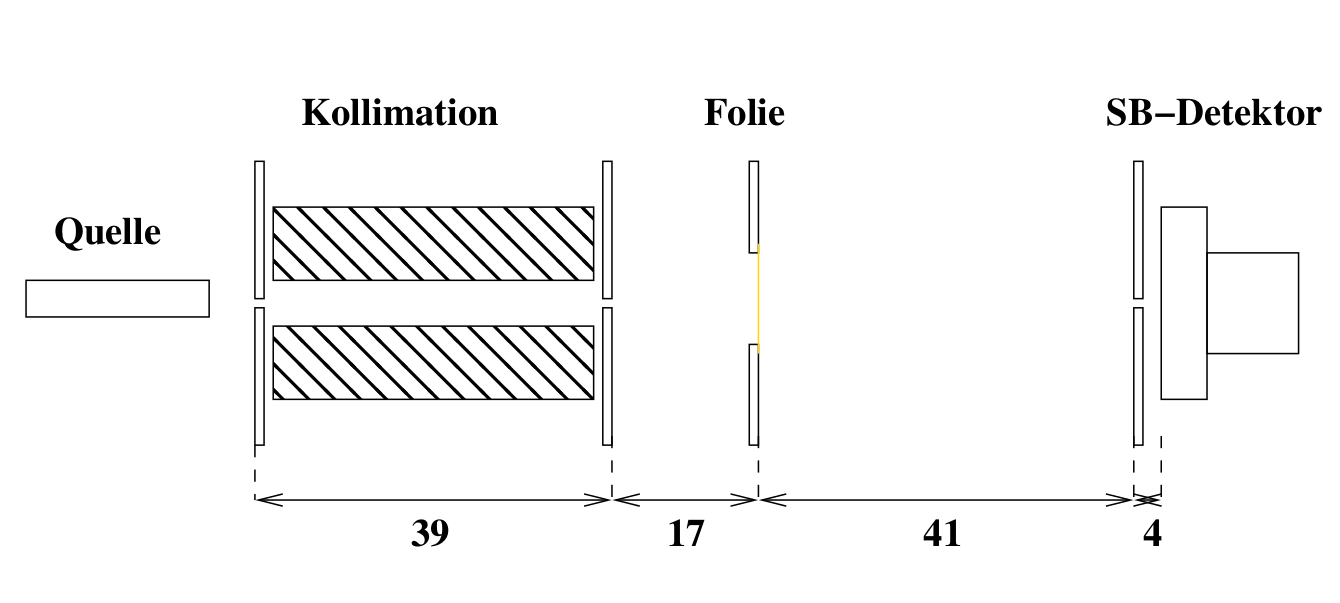
\includegraphics[width=1\textwidth]{ressources/aufbau.png}
   \caption{Schematischer Versuchsaufbau. Alle Abmessungen sind in der Einheit mm angegeben.\cite{skript}}
   \label{aufbau}
 \end{figure}
Aufgrund der geringen Reichweite der $\alpha$-Teilchen befindet sich die
ganze Apparatur im Vakuum. Zur Auslese des Detektors wird ein
Verstärker und ein Speicheroszilloskop verwendet.

